\section{Ray Tracing}

To make a better model we first need to understand how light works.  In the real world a light source emits photons that collide with an object, which changes the energy state of the photon.  This photon is then reflected off the object and then enters our eyes, which our brain then interprets as a color.  One problem with this modelling is that only a small percent of emitted light is actually seen.  A better more efficient solution exists in using ray tracing.  

Ray tracing model realistic light by tracing photons that enter the eye back the light source.  Each photon can be computed independently which making ray tracing inherently parallel.  An initial point is used as the focal point, again known as the \textit{eye}.  A photon is traced backwards from the eye through an image plane in front of the eye.  This image plane acts like film in a pinhole camera.  

\begin{figure}[H]
\begin{center}
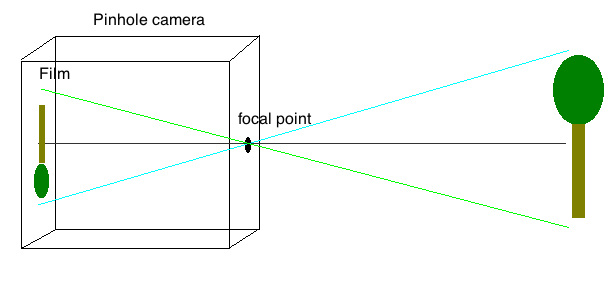
\includegraphics[scale=0.6]{pineholecamera.png} 
\caption{Pinhole camera}
\label{pinhole-camera}
\end{center}
\end{figure}

In a pinhole camera the image is upside down on the film; photons pass through the focal point and cross the central plain.  The camera can be simplified by moving the film in front of the focal point.

 \begin{figure}[H]
 \begin{center}
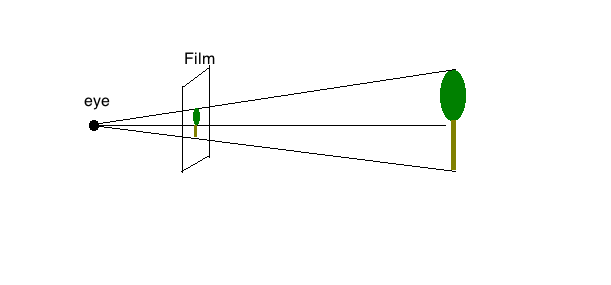
\includegraphics[scale=0.6]{raycamera.png} 
\caption{Ray tracer camera}
\label{ray-camera}
\end{center}
\end{figure}

Algorithm \ref{ray-trace} is a simple implementation producing images similar to the z-buffering algorithm.  The scene consists of a list of geometric objects.  Unlike z-buffering any shaped object can be used.  The image buffer is an array that holds the resulting output colors from the algorithm.  A ray consists of a starting vector and a normalized direction vector.  A ray is created at the eye/starting vector in the direction of each pixel in the image plane.  The pixel is set to the color of the closest object that collides with the ray.  

\begin{algorithm}[H]
\begin{algorithmic}[1]
\STATE $O[ ] \gets \textit{All objects in scene}$ 
\STATE $I[] \gets 0$ \COMMENT{Clear image buffer}
\STATE
\FOR{ each pixel p in I }
	\STATE $I_{p} \gets raytrace( castray( eye, p ))$
\ENDFOR
\STATE 
\STATE \textit{color} \textbf{function} raytrace(  R )
	\STATE $c  \gets \textit{ambient color } $
	\STATE $d \gets \infty $
	\FOR{ each object o in O[] }
		\IF{ collision( R, o )  }
			\IF{ $distance( \textit{eye}, o ) < d$ }
				\STATE $d \gets distance( \textit{eye}, o )$
				\STATE $c \gets color( o )$
			\ENDIF
		\ENDIF
	\ENDFOR
	\STATE \textbf{return} c

\end{algorithmic}
\caption{Simple ray tracing algorithm.}
\label{ray-trace}
\end{algorithm}

Adding light and shadow with this algorithm is done by computing the amount of light at each point of collision.  A ray is cast from each collision point to every light source in the scene.  Any object between the collision point and the light is in shadow.   It does not get light added to its color. If the ray's closest collision is with the light source then the point's color is computed.  A point's color is computed from three components: \textit{ambient}, \textit{diffuse}, and \textit{specular} lighting\cite{kalinini:2008}.

Surfaces can be made reflective or refractive by using recursion.  If a surface is reflective a new ray is computed at the point of collision.   The surface normal at that point  is used as a reflection plane to create the reflected ray.  This new ray is used to compute reflected color.  This produces shiny surfaces and mirrors.  

Refraction is handled in the same way with the exception of the way the refracted ray is computed.  Refracted rays are bent into the object.  The angle depends on the properties of the object's material.  Light passing through transparent materials like glass and water. Algorithm \ref{ray-trace-full} shows an example program using lighting, reflections, and refractions.
  
\begin{algorithm}[H]
\begin{algorithmic}[1]
\STATE $O[\ ] \gets \textit{All objects in scene}$ 
\STATE $L[\ ] \gets \textit{All lights in scene}$
\STATE $I[\ ] \gets 0$ \COMMENT{Clear image buffer}
\STATE
\FOR{ each pixel p in I }
	\STATE $I_{p} \gets raytrace( castray( eye, p ))$
\ENDFOR
\STATE 
\STATE \textit{color} \textbf{function} raytrace(  R, depth )
	\STATE $c  \gets \textit{ambient color } $
	\STATE $d \gets \infty $
	\STATE $s \gets \textit{NULL}$
	\FOR{ each object o in O[] }
		\IF{ collision( R, o )  }
			\IF{ $distance( \textit{eye}, o ) < d$ }
				\STATE $d \gets distance( \textit{eye}, o )$
				\STATE $s \gets o$
			\ENDIF
		\ENDIF
	\ENDFOR
	\IF{ $s\ \textbf{NOT}\ \textit{NULL}$ }
		\STATE \COMMENT{Find direct light on object s}
		\STATE $pi \gets pointOfCollision( R, s )$
		\FOR{ each light l in L }
			\STATE $lr \gets castRay( pi, l )$
			\STATE $ld \gets distance( pi, l )$
			\STATE $shade \gets 1$
			\FOR{ each object o in O }
				\IF{ collision( lr, o ) \textbf{AND} distance( lr, o ) < ld }
					\STATE $shade \gets 0$				
				\ENDIF
				\STATE $c \gets c +( diffuse( s, l ) + specular( s, l )) * shade$ 
			\ENDFOR
		\ENDFOR
		\STATE \COMMENT{Recursively compute reflections}
		\IF{ $reflectivity( s ) > 0\ \textbf{AND}\ depth < depthMax$ }
			\STATE $rr \gets reflection( pi, normal( s, pi ))$
			\STATE $c \gets c + raytrace( rr ) * reflectivity( s )$
		\ENDIF
		\STATE \COMMENT{Recursively compute refraction}
		\IF{ $transparency( s ) > 0\ \textbf{AND}\ depth < depthMax$ }
			\STATE $rr \gets refraction( pi, normal( s, pi ), s )$
			\STATE $c \gets c + raytrace( rr ) * transparency( s )$
		\ENDIF
	\ENDIF
	\STATE \textbf{return} c

\end{algorithmic}
\caption{ Ray tracing algorithm with lighting. }
\label{ray-trace-full}
\end{algorithm}
\newpage

Images produced with this algorithm tend to have overly sharp edges between objects and shadows, and pixelation.  Anti-aliasing is used to reduce jagged edges and pixelated objects. Soft shadows reduces the sharp transition from light to shadow.

Anti-aliasing is done by casting more rays through a pixel and averaging the resulting colors.  The area in space a pixel occupies is subdivided into smaller regions.  Rays are cast from the eye through these regions.  Rays can be cast through the center for a shaper image, or randomly for softer edges.  Anti-aliasing can increase the computation cost dramatically.  Each new ray can create two new rays for reflection and refraction.

\begin{figure}[H]
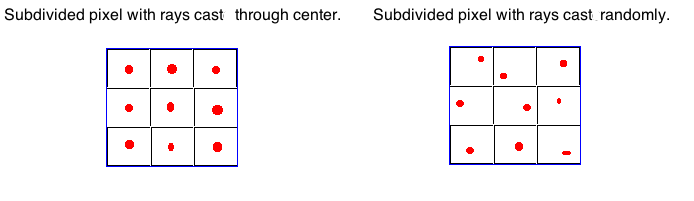
\includegraphics[scale=0.6]{aa.png} 
\caption{Anti-aliasing for a single pixel.}
\label{aa}
\end{figure}

 The simple lighting model casts a ray from the point of collision to the center of a light source, however points on the edge of a shadow may be in partial light.  In the real world a light bulb has volume unlike a single point.  A soft shadow is computed by casting several rays from the collision point to a point in the light's volume, the results are averaged to computer the final color.  These rays are often cast randomly through a uniform subdivision of the light source's volume.  Most ray tracers only use soft shadowing on simple shapes like planes and polygons.  Soft shadows can be expensive to compute because each light ray needs to be tested if it is blocked by an object.

\begin{figure}[H]
\begin{center}
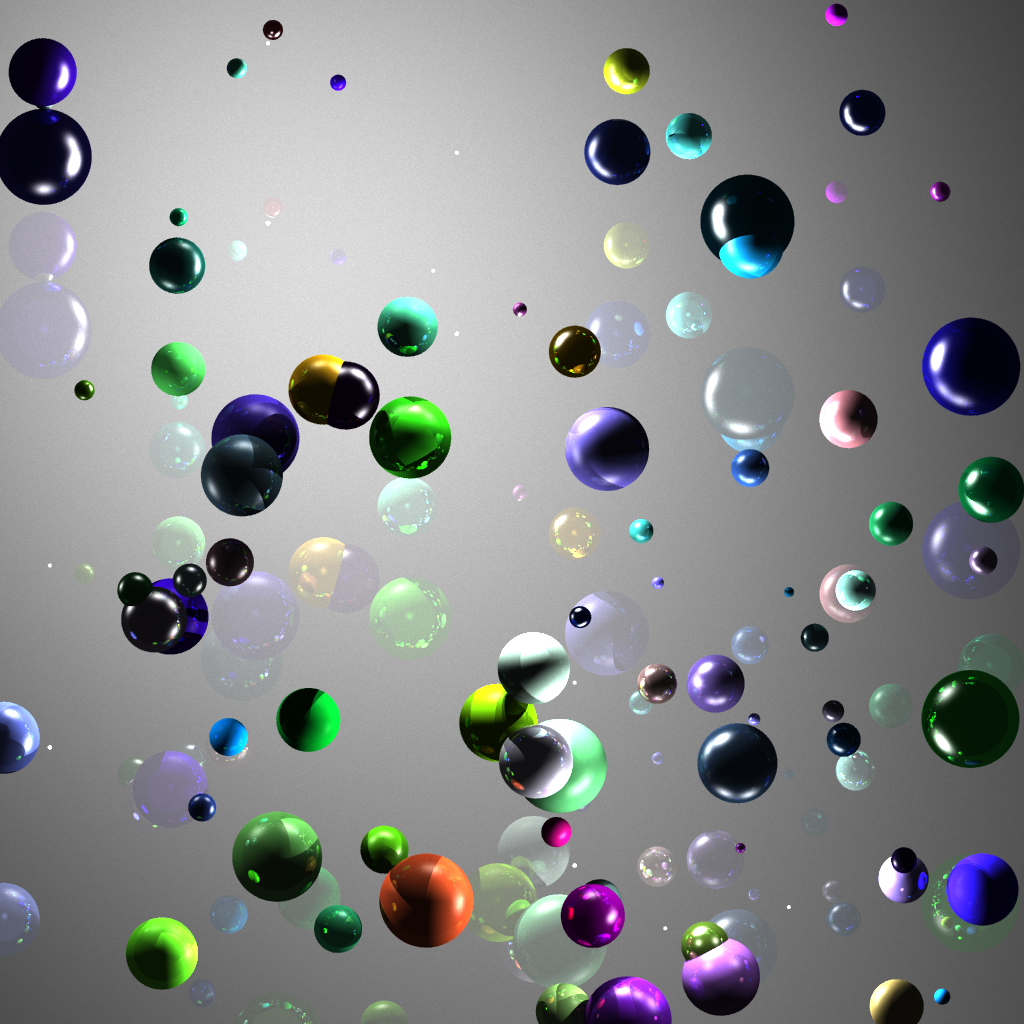
\includegraphics[scale=0.21]{result1.png} 
\caption{Non-optimized ray-traced image with eight light sources, and eighty spheres.  Rendering time was thirty-four minutes .}
\label{result1}
\end{center}
\end{figure}

